\documentclass[twoside]{book}

% Packages required by doxygen
\usepackage{fixltx2e}
\usepackage{calc}
\usepackage{doxygen}
\usepackage[export]{adjustbox} % also loads graphicx
\usepackage{graphicx}
\usepackage[utf8]{inputenc}
\usepackage{makeidx}
\usepackage{multicol}
\usepackage{multirow}
\PassOptionsToPackage{warn}{textcomp}
\usepackage{textcomp}
\usepackage[nointegrals]{wasysym}
\usepackage[table]{xcolor}

% Font selection
\usepackage[T1]{fontenc}
\usepackage[scaled=.90]{helvet}
\usepackage{courier}
\usepackage{amssymb}
\usepackage{sectsty}
\renewcommand{\familydefault}{\sfdefault}
\allsectionsfont{%
  \fontseries{bc}\selectfont%
  \color{darkgray}%
}
\renewcommand{\DoxyLabelFont}{%
  \fontseries{bc}\selectfont%
  \color{darkgray}%
}
\newcommand{\+}{\discretionary{\mbox{\scriptsize$\hookleftarrow$}}{}{}}

% Page & text layout
\usepackage{geometry}
\geometry{%
  a4paper,%
  top=2.5cm,%
  bottom=2.5cm,%
  left=2.5cm,%
  right=2.5cm%
}
\tolerance=750
\hfuzz=15pt
\hbadness=750
\setlength{\emergencystretch}{15pt}
\setlength{\parindent}{0cm}
\setlength{\parskip}{0.2cm}
\makeatletter
\renewcommand{\paragraph}{%
  \@startsection{paragraph}{4}{0ex}{-1.0ex}{1.0ex}{%
    \normalfont\normalsize\bfseries\SS@parafont%
  }%
}
\renewcommand{\subparagraph}{%
  \@startsection{subparagraph}{5}{0ex}{-1.0ex}{1.0ex}{%
    \normalfont\normalsize\bfseries\SS@subparafont%
  }%
}
\makeatother

% Headers & footers
\usepackage{fancyhdr}
\pagestyle{fancyplain}
\fancyhead[LE]{\fancyplain{}{\bfseries\thepage}}
\fancyhead[CE]{\fancyplain{}{}}
\fancyhead[RE]{\fancyplain{}{\bfseries\leftmark}}
\fancyhead[LO]{\fancyplain{}{\bfseries\rightmark}}
\fancyhead[CO]{\fancyplain{}{}}
\fancyhead[RO]{\fancyplain{}{\bfseries\thepage}}
\fancyfoot[LE]{\fancyplain{}{}}
\fancyfoot[CE]{\fancyplain{}{}}
\fancyfoot[RE]{\fancyplain{}{\bfseries\scriptsize Generated on Mon Nov 16 2015 16\+:42\+:25 for Prototype Serialization and testing by Doxygen }}
\fancyfoot[LO]{\fancyplain{}{\bfseries\scriptsize Generated on Mon Nov 16 2015 16\+:42\+:25 for Prototype Serialization and testing by Doxygen }}
\fancyfoot[CO]{\fancyplain{}{}}
\fancyfoot[RO]{\fancyplain{}{}}
\renewcommand{\footrulewidth}{0.4pt}
\renewcommand{\chaptermark}[1]{%
  \markboth{#1}{}%
}
\renewcommand{\sectionmark}[1]{%
  \markright{\thesection\ #1}%
}

% Indices & bibliography
\usepackage{natbib}
\usepackage[titles]{tocloft}
\setcounter{tocdepth}{3}
\setcounter{secnumdepth}{5}
\makeindex

% Hyperlinks (required, but should be loaded last)
\usepackage{ifpdf}
\ifpdf
  \usepackage[pdftex,pagebackref=true]{hyperref}
\else
  \usepackage[ps2pdf,pagebackref=true]{hyperref}
\fi
\hypersetup{%
  colorlinks=true,%
  linkcolor=blue,%
  citecolor=blue,%
  unicode%
}

% Custom commands
\newcommand{\clearemptydoublepage}{%
  \newpage{\pagestyle{empty}\cleardoublepage}%
}


%===== C O N T E N T S =====

\begin{document}

% Titlepage & ToC
\hypersetup{pageanchor=false,
             bookmarks=true,
             bookmarksnumbered=true,
             pdfencoding=unicode
            }
\pagenumbering{roman}
\begin{titlepage}
\vspace*{7cm}
\begin{center}%
{\Large Prototype Serialization and testing \\[1ex]\large Version 1.\+0 }\\
\vspace*{1cm}
{\large Generated by Doxygen 1.8.10}\\
\vspace*{0.5cm}
{\small Mon Nov 16 2015 16:42:25}\\
\end{center}
\end{titlepage}
\clearemptydoublepage
\tableofcontents
\clearemptydoublepage
\pagenumbering{arabic}
\hypersetup{pageanchor=true}

%--- Begin generated contents ---
\chapter{Hierarchical Index}
\section{Class Hierarchy}
This inheritance list is sorted roughly, but not completely, alphabetically\+:\begin{DoxyCompactList}
\item \contentsline{section}{Equipment}{\pageref{class_equipment}}{}
\begin{DoxyCompactList}
\item \contentsline{section}{Benchpress}{\pageref{class_benchpress}}{}
\item \contentsline{section}{Legpress}{\pageref{class_legpress}}{}
\end{DoxyCompactList}
\item \contentsline{section}{Factory}{\pageref{class_factory}}{}
\end{DoxyCompactList}

\chapter{Class Index}
\section{Class List}
Here are the classes, structs, unions and interfaces with brief descriptions\+:\begin{DoxyCompactList}
\item\contentsline{section}{\hyperlink{class_benchpress}{Benchpress} }{\pageref{class_benchpress}}{}
\item\contentsline{section}{\hyperlink{class_equipment}{Equipment} }{\pageref{class_equipment}}{}
\item\contentsline{section}{\hyperlink{class_factory}{Factory} }{\pageref{class_factory}}{}
\item\contentsline{section}{\hyperlink{class_legpress}{Legpress} }{\pageref{class_legpress}}{}
\end{DoxyCompactList}

\chapter{Class Documentation}
\hypertarget{class_benchpress}{}\section{Benchpress Class Reference}
\label{class_benchpress}\index{Benchpress@{Benchpress}}
Inheritance diagram for Benchpress\+:\begin{figure}[H]
\begin{center}
\leavevmode
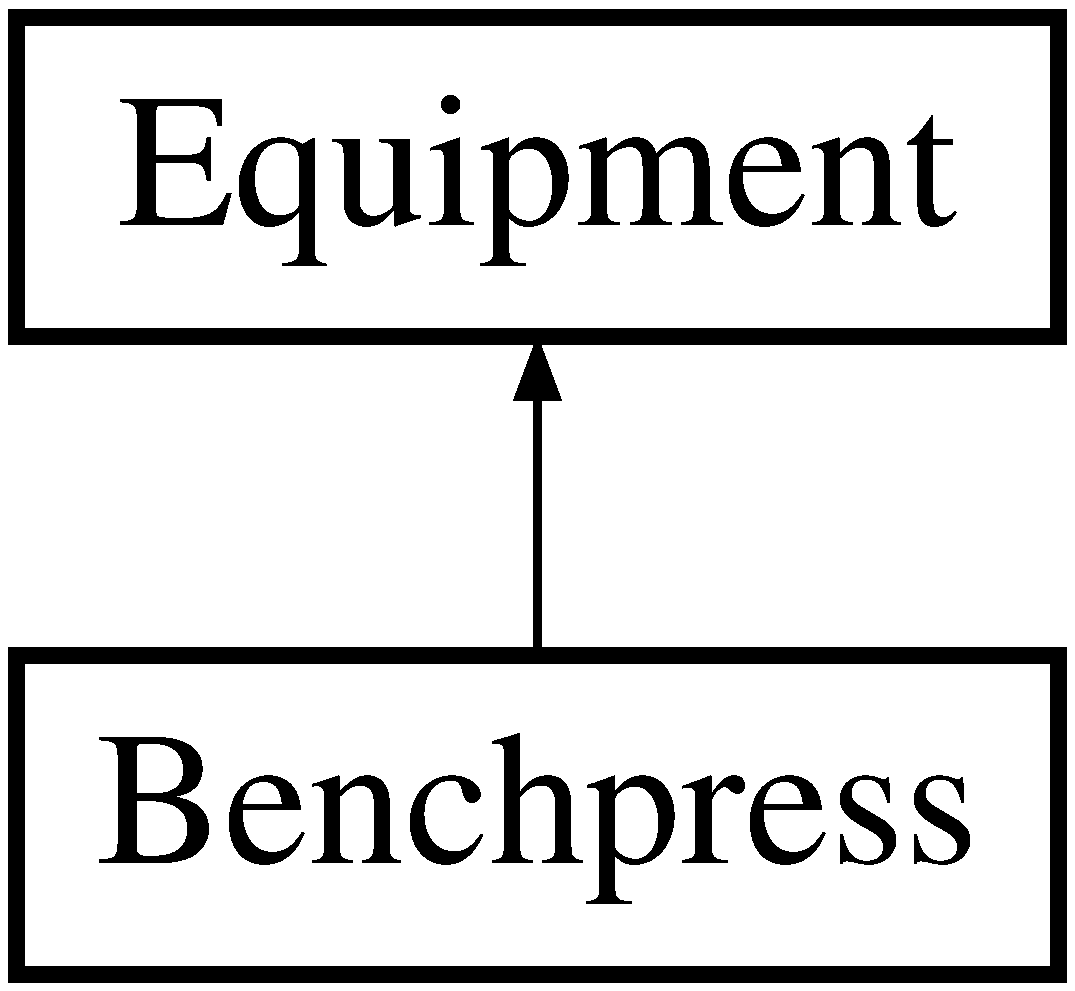
\includegraphics[height=2.000000cm]{class_benchpress}
\end{center}
\end{figure}
\subsection*{Public Member Functions}
\begin{DoxyCompactItemize}
\item 
\hyperlink{class_equipment}{Equipment} $\ast$ \hyperlink{class_benchpress_abf49fcc927642b404b3a6b9f4a62f10e}{clone} ()
\item 
void \hyperlink{class_benchpress_a47d7accc61f6322cda33c3eca84d11cd}{print\+Equipment} ()
\end{DoxyCompactItemize}
\subsection*{Additional Inherited Members}


\subsection{Member Function Documentation}
\hypertarget{class_benchpress_abf49fcc927642b404b3a6b9f4a62f10e}{}\index{Benchpress@{Benchpress}!clone@{clone}}
\index{clone@{clone}!Benchpress@{Benchpress}}
\subsubsection[{clone()}]{\setlength{\rightskip}{0pt plus 5cm}{\bf Equipment}$\ast$ Benchpress\+::clone (
\begin{DoxyParamCaption}
{}
\end{DoxyParamCaption}
)\hspace{0.3cm}{\ttfamily [inline]}, {\ttfamily [virtual]}}\label{class_benchpress_abf49fcc927642b404b3a6b9f4a62f10e}
Returns a clone 

Implements \hyperlink{class_equipment_a866383329b92e50a2c323e05e55fa948}{Equipment}.

\hypertarget{class_benchpress_a47d7accc61f6322cda33c3eca84d11cd}{}\index{Benchpress@{Benchpress}!print\+Equipment@{print\+Equipment}}
\index{print\+Equipment@{print\+Equipment}!Benchpress@{Benchpress}}
\subsubsection[{print\+Equipment()}]{\setlength{\rightskip}{0pt plus 5cm}void Benchpress\+::print\+Equipment (
\begin{DoxyParamCaption}
{}
\end{DoxyParamCaption}
)\hspace{0.3cm}{\ttfamily [inline]}, {\ttfamily [virtual]}}\label{class_benchpress_a47d7accc61f6322cda33c3eca84d11cd}
prints the instance type and instance name 

Implements \hyperlink{class_equipment_a12b5c474bf74a6f2272f02d0a745b41d}{Equipment}.



The documentation for this class was generated from the following file\+:\begin{DoxyCompactItemize}
\item 
V\+S\+Proj/\+V\+S\+Proj/V\+S\+Proj.\+cpp\end{DoxyCompactItemize}

\hypertarget{class_equipment}{}\section{Equipment Class Reference}
\label{class_equipment}\index{Equipment@{Equipment}}
Inheritance diagram for Equipment\+:\begin{figure}[H]
\begin{center}
\leavevmode
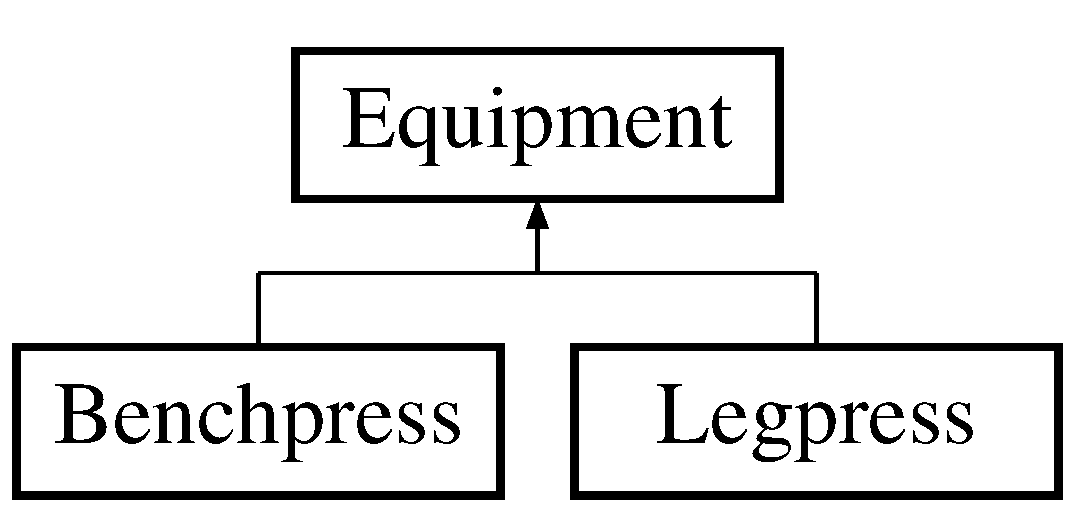
\includegraphics[height=2.000000cm]{class_equipment}
\end{center}
\end{figure}
\subsection*{Public Member Functions}
\begin{DoxyCompactItemize}
\item 
virtual \hyperlink{class_equipment}{Equipment} $\ast$ \hyperlink{class_equipment_a866383329b92e50a2c323e05e55fa948}{clone} ()=0
\item 
virtual void \hyperlink{class_equipment_a12b5c474bf74a6f2272f02d0a745b41d}{print\+Equipment} ()=0
\item 
\hypertarget{class_equipment_a719429595638879fd91d7205097ab118}{}virtual string {\bfseries get\+Equipment\+Type} ()\label{class_equipment_a719429595638879fd91d7205097ab118}

\item 
rapidjson\+::\+Document \hyperlink{class_equipment_aa398c2e8e7b46534b8284788c30cf45e}{serialize} ()
\end{DoxyCompactItemize}
\subsection*{Public Attributes}
\begin{DoxyCompactItemize}
\item 
string \hyperlink{class_equipment_a65c3c95bb543fd763fe6bdf7587c1d33}{name} = \char`\"{}Unnamed\char`\"{}
\end{DoxyCompactItemize}


\subsection{Detailed Description}
\hyperlink{class_equipment}{Equipment} is the base class for several subclasses. 

\subsection{Member Function Documentation}
\hypertarget{class_equipment_a866383329b92e50a2c323e05e55fa948}{}\index{Equipment@{Equipment}!clone@{clone}}
\index{clone@{clone}!Equipment@{Equipment}}
\subsubsection[{clone()=0}]{\setlength{\rightskip}{0pt plus 5cm}virtual {\bf Equipment}$\ast$ Equipment\+::clone (
\begin{DoxyParamCaption}
{}
\end{DoxyParamCaption}
)\hspace{0.3cm}{\ttfamily [pure virtual]}}\label{class_equipment_a866383329b92e50a2c323e05e55fa948}
All subclasses of \hyperlink{class_equipment}{Equipment} must have clone functionality 

Implemented in \hyperlink{class_benchpress_abf49fcc927642b404b3a6b9f4a62f10e}{Benchpress}, and \hyperlink{class_legpress_afe01d06ba0de89e04eb2f8cf405edefd}{Legpress}.

\hypertarget{class_equipment_a12b5c474bf74a6f2272f02d0a745b41d}{}\index{Equipment@{Equipment}!print\+Equipment@{print\+Equipment}}
\index{print\+Equipment@{print\+Equipment}!Equipment@{Equipment}}
\subsubsection[{print\+Equipment()=0}]{\setlength{\rightskip}{0pt plus 5cm}virtual void Equipment\+::print\+Equipment (
\begin{DoxyParamCaption}
{}
\end{DoxyParamCaption}
)\hspace{0.3cm}{\ttfamily [pure virtual]}}\label{class_equipment_a12b5c474bf74a6f2272f02d0a745b41d}
prints the instance type and instance name 

Implemented in \hyperlink{class_benchpress_a47d7accc61f6322cda33c3eca84d11cd}{Benchpress}, and \hyperlink{class_legpress_aab4968ff900ea7a789e883ae33042d13}{Legpress}.

\hypertarget{class_equipment_aa398c2e8e7b46534b8284788c30cf45e}{}\index{Equipment@{Equipment}!serialize@{serialize}}
\index{serialize@{serialize}!Equipment@{Equipment}}
\subsubsection[{serialize()}]{\setlength{\rightskip}{0pt plus 5cm}rapidjson\+::\+Document Equipment\+::serialize (
\begin{DoxyParamCaption}
{}
\end{DoxyParamCaption}
)\hspace{0.3cm}{\ttfamily [inline]}}\label{class_equipment_aa398c2e8e7b46534b8284788c30cf45e}
returns the instance type as string serializes the data inside the object 

\subsection{Member Data Documentation}
\hypertarget{class_equipment_a65c3c95bb543fd763fe6bdf7587c1d33}{}\index{Equipment@{Equipment}!name@{name}}
\index{name@{name}!Equipment@{Equipment}}
\subsubsection[{name}]{\setlength{\rightskip}{0pt plus 5cm}string Equipment\+::name = \char`\"{}Unnamed\char`\"{}}\label{class_equipment_a65c3c95bb543fd763fe6bdf7587c1d33}
Name of equipments instance, by default equipment is unnamed 

The documentation for this class was generated from the following file\+:\begin{DoxyCompactItemize}
\item 
C\+:/\+Users/\+Anthony/\+Documents/\+Seng330-\/\+Ass2-\/\+Protoype-\/protocol-\/doxygen-\/testing/\+V\+S\+Proj/\+V\+S\+Proj/V\+S\+Proj.\+cpp\end{DoxyCompactItemize}

\hypertarget{class_factory}{}\section{Factory Class Reference}
\label{class_factory}\index{Factory@{Factory}}
\subsection*{Static Public Member Functions}
\begin{DoxyCompactItemize}
\item 
static \hyperlink{class_equipment}{Equipment} $\ast$ \hyperlink{class_factory_a616390c764e9f194c46f82f79ba94393}{make\+\_\+\+Equipment} (int choice, string name)
\begin{DoxyCompactList}\small\item\em A prototype creation Method taking two arguments and returning an class of Equipment$\ast$ type. \end{DoxyCompactList}\end{DoxyCompactItemize}


\subsection{Detailed Description}
\hyperlink{class_factory}{Factory}, holds a series of registered prototype classes. These classes are all subclasses of \hyperlink{class_equipment}{Equipment}. \hyperlink{class_factory}{Factory} is used to generate new instances with clone() 

\subsection{Member Function Documentation}
\hypertarget{class_factory_a616390c764e9f194c46f82f79ba94393}{}\index{Factory@{Factory}!make\+\_\+\+Equipment@{make\+\_\+\+Equipment}}
\index{make\+\_\+\+Equipment@{make\+\_\+\+Equipment}!Factory@{Factory}}
\subsubsection[{make\+\_\+\+Equipment(int choice, string name)}]{\setlength{\rightskip}{0pt plus 5cm}{\bf Equipment} $\ast$ Factory\+::make\+\_\+\+Equipment (
\begin{DoxyParamCaption}
\item[{int}]{choice, }
\item[{string}]{name}
\end{DoxyParamCaption}
)\hspace{0.3cm}{\ttfamily [static]}}\label{class_factory_a616390c764e9f194c46f82f79ba94393}


A prototype creation Method taking two arguments and returning an class of Equipment$\ast$ type. 


\begin{DoxyParams}{Parameters}
{\em choice} & an integer argument Indicating which registered prototype to use. \\
\hline
{\em name} & used to set the instance name of the newly generated object. \\
\hline
\end{DoxyParams}
\begin{DoxyReturn}{Returns}
the new prototyped object, with instance name set.\+All subclasses of \hyperlink{class_equipment}{Equipment} must have clone functionality 
\end{DoxyReturn}


The documentation for this class was generated from the following file\+:\begin{DoxyCompactItemize}
\item 
C\+:/\+Users/\+Anthony/\+Documents/\+Seng330-\/\+Ass2-\/\+Protoype-\/protocol-\/doxygen-\/testing/\+V\+S\+Proj/\+V\+S\+Proj/V\+S\+Proj.\+cpp\end{DoxyCompactItemize}

\hypertarget{class_legpress}{}\section{Legpress Class Reference}
\label{class_legpress}\index{Legpress@{Legpress}}
Inheritance diagram for Legpress\+:\begin{figure}[H]
\begin{center}
\leavevmode
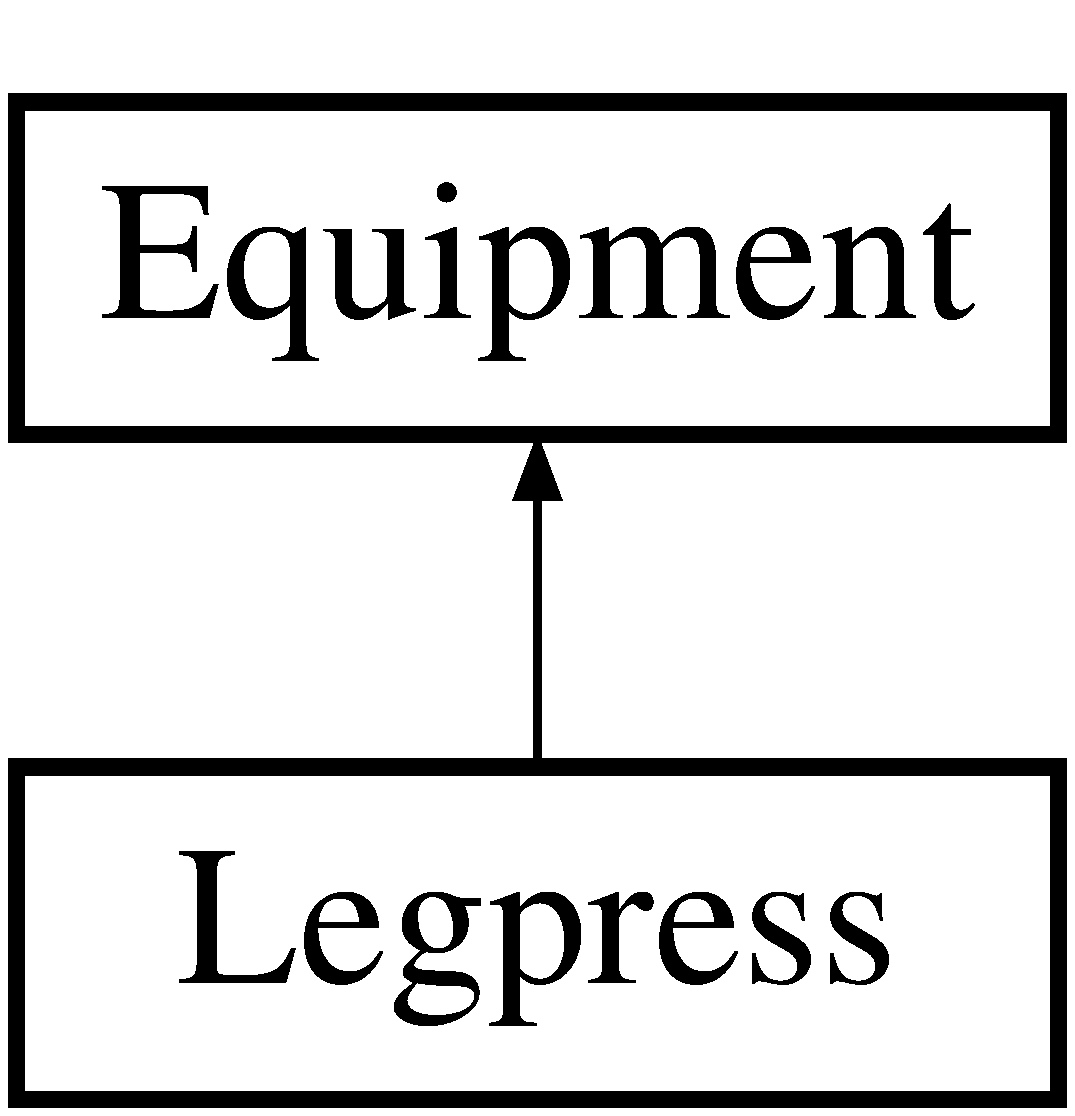
\includegraphics[height=2.000000cm]{class_legpress}
\end{center}
\end{figure}
\subsection*{Public Member Functions}
\begin{DoxyCompactItemize}
\item 
\hyperlink{class_equipment}{Equipment} $\ast$ \hyperlink{class_legpress_afe01d06ba0de89e04eb2f8cf405edefd}{clone} ()
\item 
string \hyperlink{class_legpress_a53ae3609c10adb7731b8881713d73c1e}{get\+Equipment\+Type} ()
\item 
void \hyperlink{class_legpress_aab4968ff900ea7a789e883ae33042d13}{print\+Equipment} ()
\end{DoxyCompactItemize}
\subsection*{Additional Inherited Members}


\subsection{Detailed Description}
\hyperlink{class_legpress}{Legpress} is a subclass of \hyperlink{class_equipment}{Equipment}. 

\subsection{Member Function Documentation}
\hypertarget{class_legpress_afe01d06ba0de89e04eb2f8cf405edefd}{}\index{Legpress@{Legpress}!clone@{clone}}
\index{clone@{clone}!Legpress@{Legpress}}
\subsubsection[{clone()}]{\setlength{\rightskip}{0pt plus 5cm}{\bf Equipment}$\ast$ Legpress\+::clone (
\begin{DoxyParamCaption}
{}
\end{DoxyParamCaption}
)\hspace{0.3cm}{\ttfamily [inline]}, {\ttfamily [virtual]}}\label{class_legpress_afe01d06ba0de89e04eb2f8cf405edefd}
All subclasses of \hyperlink{class_equipment}{Equipment} must have clone functionality 

Implements \hyperlink{class_equipment_a866383329b92e50a2c323e05e55fa948}{Equipment}.

\hypertarget{class_legpress_a53ae3609c10adb7731b8881713d73c1e}{}\index{Legpress@{Legpress}!get\+Equipment\+Type@{get\+Equipment\+Type}}
\index{get\+Equipment\+Type@{get\+Equipment\+Type}!Legpress@{Legpress}}
\subsubsection[{get\+Equipment\+Type()}]{\setlength{\rightskip}{0pt plus 5cm}string Legpress\+::get\+Equipment\+Type (
\begin{DoxyParamCaption}
{}
\end{DoxyParamCaption}
)\hspace{0.3cm}{\ttfamily [inline]}, {\ttfamily [virtual]}}\label{class_legpress_a53ae3609c10adb7731b8881713d73c1e}
Returns a clone 

Reimplemented from \hyperlink{class_equipment}{Equipment}.

\hypertarget{class_legpress_aab4968ff900ea7a789e883ae33042d13}{}\index{Legpress@{Legpress}!print\+Equipment@{print\+Equipment}}
\index{print\+Equipment@{print\+Equipment}!Legpress@{Legpress}}
\subsubsection[{print\+Equipment()}]{\setlength{\rightskip}{0pt plus 5cm}void Legpress\+::print\+Equipment (
\begin{DoxyParamCaption}
{}
\end{DoxyParamCaption}
)\hspace{0.3cm}{\ttfamily [inline]}, {\ttfamily [virtual]}}\label{class_legpress_aab4968ff900ea7a789e883ae33042d13}
prints the instance type and instance name 

Implements \hyperlink{class_equipment_a12b5c474bf74a6f2272f02d0a745b41d}{Equipment}.



The documentation for this class was generated from the following file\+:\begin{DoxyCompactItemize}
\item 
C\+:/\+Users/\+Anthony/\+Documents/\+Seng330-\/\+Ass2-\/\+Protoype-\/protocol-\/doxygen-\/testing/\+V\+S\+Proj/\+V\+S\+Proj/V\+S\+Proj.\+cpp\end{DoxyCompactItemize}

%--- End generated contents ---

% Index
\backmatter
\newpage
\phantomsection
\clearemptydoublepage
\addcontentsline{toc}{chapter}{Index}
\printindex

\end{document}
